\documentclass{article}
    \usepackage{amssymb}
    \usepackage{color}
    \usepackage{listings}
    \usepackage{graphicx}
    \usepackage{subcaption}
    \usepackage{geometry}
    \usepackage{float}
    \usepackage{caption}
    \usepackage{blindtext}
    \usepackage{url}
    \geometry{
    a4paper,
    total={170mm,257mm},
    left=20mm,
    top=20mm,
    }
    \DeclareCaptionFormat{citation}{%
    \ifx\captioncitation\relax\relax\else
      \captioncitation\par
    \fi
    #1#2#3\par}
 \newcommand*\setcaptioncitation[1]{\def\captioncitation{\textit{Source:}~#1}}
 \let\captioncitation\relax
 \captionsetup{format=citation,justification=centering}
  \setlength{\parindent}{0em}
    \setlength{\parskip}{1em} % length of the spacing
    
    \definecolor{gray}{rgb}{0.4,0.4,0.4}
    \definecolor{darkblue}{rgb}{0.0,0.0,0.6}
    \definecolor{cyan}{rgb}{0.0,0.6,0.6}
    \definecolor{lightgray}{rgb}{.9,.9,.9}
	\definecolor{darkgray}{rgb}{.4,.4,.4}
	\definecolor{purple}{rgb}{0.65, 0.12, 0.82}
    \lstset{
      basicstyle=\ttfamily,
      frame=tb,
      tabsize=2,
      columns=fixed,
      showstringspaces=false,
      commentstyle=\color{gray}\upshape
      frame=lr,
      framesep=8pt,
      framerule=0pt,
    }

    \lstset{ % General setup for the package
        language=Python,
        basicstyle=\small\sffamily,
        numbers=left,
        numberstyle=\tiny,
        frame=tb,
        tabsize=4,
        columns=fixed,
        showstringspaces=false,
        showtabs=false,
        keepspaces,
        commentstyle=\color{red},
        keywordstyle=\color{blue},
        emphstyle=\ttb\color{deepred},    
        stringstyle=\color{blue}
    }

    
    
    \begin{document}

    \begin{titlepage}
        \begin{center}
            \vspace*{1cm}
            \begin{figure}
                \centering
                
\includegraphics[width=0.5\linewidth]{./img/vub.png}
            \end{figure}
            \Huge
            \textbf{Data Representation,Reduction and Analysis}
            
           
            
            \vspace{1.5cm}

            \textbf {\centering Juan Jose Soriano Escobar}
            \vspace{0.5cm}
            \newline
            \textbf{\centering Redona Brahimetaj}
            \vspace{0.5cm}
            \vfill
            
            
            \Large
            Master in Applied Computer Science and Engineering\\
            Vrije Universiteit Brussels\\
            Brussels Belgium\\
            January 15, 2017
            
        \end{center}
    \end{titlepage}

    \newpage

    \begin{appendix}
        \listoffigures
      \end{appendix}
      \newpage


        \section{Introduction}
        Massive amounts of data are constantly harvested from diverse information sources in various domains, ranging from science and technology to business and telecommunications. Petabytes of high-dimensional data from multimodal imaging systems, social media, recommender systems, and large-scale research experiments, all require sophisticated solutions to information representation, dimensionality-reduction, and data analysis. 
        
        This project will show clearly the hidden values that stand behind data that at the first sight, look like they are not connected at all to each other. By doing the right Data cleaning, we will prove that from simple and messy data, you can extract helpful information regarding to what you want to do and the purpose why you need to do so. 
        
        In this project we were asked to do detailed analysis of the data in order to cluster them together by using K-Means and DBSCAN alogorithms. After running the algorithms in the pre-processed data, we also will visualize the results.
         
        \newpage         
        \section{ Cleaning of Tweets }
One of the most crucial parts to start with and that has a big influence in the result of our project, is data processing step. A csv file containing 2000 tweets was provided.It was required to pre-process the data to make them good enough for the 'learning' step. Below we will provide more details regarding the way how we cleaned the data. 
        
        \subsection{Pre-Processing}

        We cleaned the data by applying several filters to them. We would like to mention that for this part, we have adapted the code that we already did before on Distributed Computing and Storage Architecture project. 
        The first filtering process we did was tokenization. We chopped the data provided into small pieces so that after it would be easier to remove the stop-words like determiners, the coordinating conjunctions and prepositions.
         Another pre-processing step that we did was trying to keep only the root of the words by applying stemming. In this way the clusters would be correctly implemented since it would be easier to cluster and find similarities between words that are the same. This is a very important part and that has a hight influence in the result. 
         Something that we would like to emphasize is the fact that we did not remove the hashtags. We consider that they are a very helpful indicator when it comes to the properly group the similar words together. Below is presented the code that shows the data-cleaning. 
         
         
        \begin{lstlisting}[language=Python, caption= Python Cleaning Function, label={lst:dataCleaning}]
from nltk.stem import WordNetLemmatizer
from nltk.tokenize import TweetTokenizer
from nltk.corpus import stopwords
tknz = TweetTokenizer()  #Tokenization
tweets = CSVHelper.load_csv("Tweets_2016London.csv") #Load the provided CSV file
clean_tweets = [] 
#specify the format of the URL so we can remove it later
url_expression = 'http[s]?[:]?//(?:[a-zA-Z]|[0-9]|[$-_@.&+]|[!*\(\),]|(?:%[0-9a-fA-F][0-9a-fA-F]))+'
#remove emojis
emoji_pattern = re.compile("["
        u"\U0001F600-\U0001F64F"  # emoticons
        u"\U0001F300-\U0001F5FF"  # symbols & pictographs
        u"\U0001F680-\U0001F6FF"  # transport & map symbols
        u"\U0001F1E0-\U0001F1FF" 
        u"\U00002600-\U000027BF"
        u"\U0001f300-\U0001f64F"
        u"\U0001f680-\U0001f6FF"
        u"\u2600-\u27BF""]+", flags=re.UNICODE)
wordnet_lemmatizer = WordNetLemmatizer()
for t in tweets:
    stop = set(stopwords.words('english')) #stop words!
    framents = tknz.tokenize(t)
    clean_fragments = []
    for f in framents:
        if f not in stop: # not included in the stop words
            f = emoji_pattern.sub(r'', f)
            f = f.lower() #lowercase fragment
            f = re.sub(r'[.,"!~_:|?\']+', '', f,flags=re.MULTILINE) # Special characters
            f =  re.sub(r'\.\.\.', '', f,flags=re.MULTILINE) # 3 dots
            f = re.sub(url_expression, '', f,flags=re.MULTILINE) # links
            f = re.sub(r'@[a-z,A-Z,0-9 ]*', '', f, flags=re.MULTILINE) #clean at person references
            f = re.sub(r'RT @[a-z,A-Z]*: ', '', f, flags=re.MULTILINE) #Remove retweets
            f = wordnet_lemmatizer.lemmatize(f)
            if f:
                clean_fragments.append(f) #we append the cleaned tweet to clean_fragment vector
    clean_tweets.append(" ".join(clean_fragments)) #append the result to clean_tweets

# Export the cleaned tweets to a new csv file.Pandas Library is used
import pandas as pd
df = pd.DataFrame(clean_array)
df.to_csv("file_path.csv")
        \end{lstlisting}

        \newpage
        \section{Noise Removal}
The data that we have in disposition, are tweets that are retrieved from people that just wrote their opinions or feelings without thinking to much on what they were writing. This means that in this dataset, the tweets contain noise and we will have to remove the noise from tweets. In order to do so, 2 implementations of different algorithms are requested, K-means and DBSCAN. 
To implement the first algorithm, we will realize the need of having a consensus-matrix so that for each time that we run the same algorithm,we will count the number of times that two data points were clustered together. In this way, at the final table we would realise that if two data points are clustered together many times, it means that they are related a lot to each other and as a result they should be on the same cluster. 

Before running the K-means algorithm, we need to represent the text documents as mutually comparable vectors as it was requested. To do so,we used the TF-IDF which ranks the importance of a string in its contextual text corpus. We carefully studied and understood how does TF-IDF works and initially we implemented it by ourselves and tested it in a simple example. We took 3 documents where we tested it. But at the end we decided to use the one that was already implemented by scikit-learn even if ours was correct as well. Below we will present the code that shows the implementation we did for it. 

\begin{lstlisting}[language=Python, caption= TF-IDF implementation, label={lst:TF-IDF}]
def tf(word, blob): # function to count the term frecuency.
    return blob.words.count(word) / len(blob.words)

def n_containing(word, bloblist): # count the word ocurance in the document list.
    return sum(1 for blob in bloblist if word in blob)

def idf(word, bloblist): #inverse document fequency.
    return math.log(len(bloblist) / (1 + n_containing(word, bloblist)))

def tfidf(word, blob, bloblist):
    return tf(word, blob) * idf(word, bloblist)
           \end{lstlisting}

After representing the tweets as mutually comparable vectors by using the TF-IDF implementation from scikit-learn, we were requested to use k-means and a consensus matrix for noise removal. As it was already mentioned, for the similarity metric we were allowed to choose either Euclidean distance or the Cosine distance. After some researches, we decided that it is better to use the cosine distance in our case. It was marked as more fast and efficient in comparison with the euclidean-distance and it was especially suggested when we have to deal with text data. Reference: https://cmry.github.io/notes/euclidean-v-cosine
We understood how the cosine distance works and after that we used the one that is already provided by scikit-learn. 

\subsection{K means}

Subsequently, we had to run the K-means algorithm. We used the code that was already provided to us but we did several modifications. We run the algorithm 9 times in order to construct our consensus matrix. For each time we run the algorithm, we will store on the consensus matrix, the number of times these nodes were matched together on the same cluster.

CODE for the K-means algorithm:

\begin{lstlisting}[language=Python, caption= K-Means Algorithm, label={lst:K-Means implementation}]
    def kmeans(X,n_clusters):
        # initialize labels and prev_labels. prev_labels will be compared with labels to check if the stopping condition
        # have been reached.
        prev_labels = np.zeros(X.shape[0])
        labels = np.zeros(X.shape[0])
        indices_results = []
        # init random indices
        indices = np.random.choice(X.shape[0], n_clusters, replace=False)
        indices_results.append(indices)
        # assign centroids using the indices
        # centroids = X[indices]
        
        # the interative algorithm goes here
        while (True):
            # calculate the distances to the centroids
            distances = get_distances(X, indices)
            print(labels, indices)
    
            # assign labels
            labels = assign_labels(distances, indices)
            
            # stopping condition
            # if np.array_equal(labels, prev_labels):
            #     break
            print(indices_results)
            print(indices_results.count(indices))
    
            if indices_results.count(indices) > 2:
                break
            
            # calculate new centroids
            for cluster_indx in range(len(indices)):
                # members = X[labels == indices[cluster_indx]]
                members = [ i  for i, x in enumerate(labels) if x == indices[cluster_indx]]
                indices[cluster_indx] = new_centroid(X, members, indices)
                #centroids[cluster_indx,:] = np.mean(members,axis=0)
            indices_results.append(indices)
            # keep the labels for next round's usage
            # prev_labels = np.argmin(distances,axis=1)
            #prev_labels = labels
            indices_results.append(indices)
        
        return labels,indices
        
    \end{lstlisting}

An important additional post-processing step that was requested, was that if a pair (i, j) of tweets did not cluster together more than 10 percent of the total number of runs, the position (i, j) in the consensus matrix is set to 0. So after we had the results of the consensus matrix, we replaced all the values '1' with '0' since we run the algorithm 11 times and approximately the value that we need to change to 0 was 1. 
The main reason why the consensus matrix is helpful for us is to detect the noise. We initially implemented a threshold value by finding the average of all the entries in the constructed consensus matrix excluding the diagonals. After doing so, we found the average of each row and in case this average was less than the threshold value, we consider this as a noise point. In this way, we would have clusters with more cleaner tweets since we are going to remove all these noise points. On each time that we run the K-Means algorithm, we will remove the points that were marked as noise from the consensus matrix. 
In order to decide for the number of cluster, we decided to compute the sum of squared error (SSE). 

SSE= $\sum\limits_{i=1}^K d(x,c_{i})^2 $

In the figure \ref{fig:elbow} we plotted the results for different \textbf{K} values and the squared sum of the distance of the different centroids to its nodes in the clusters.

\begin{figure}[H]
    \begin{subfigure} {1\textwidth}  
        \centering 
        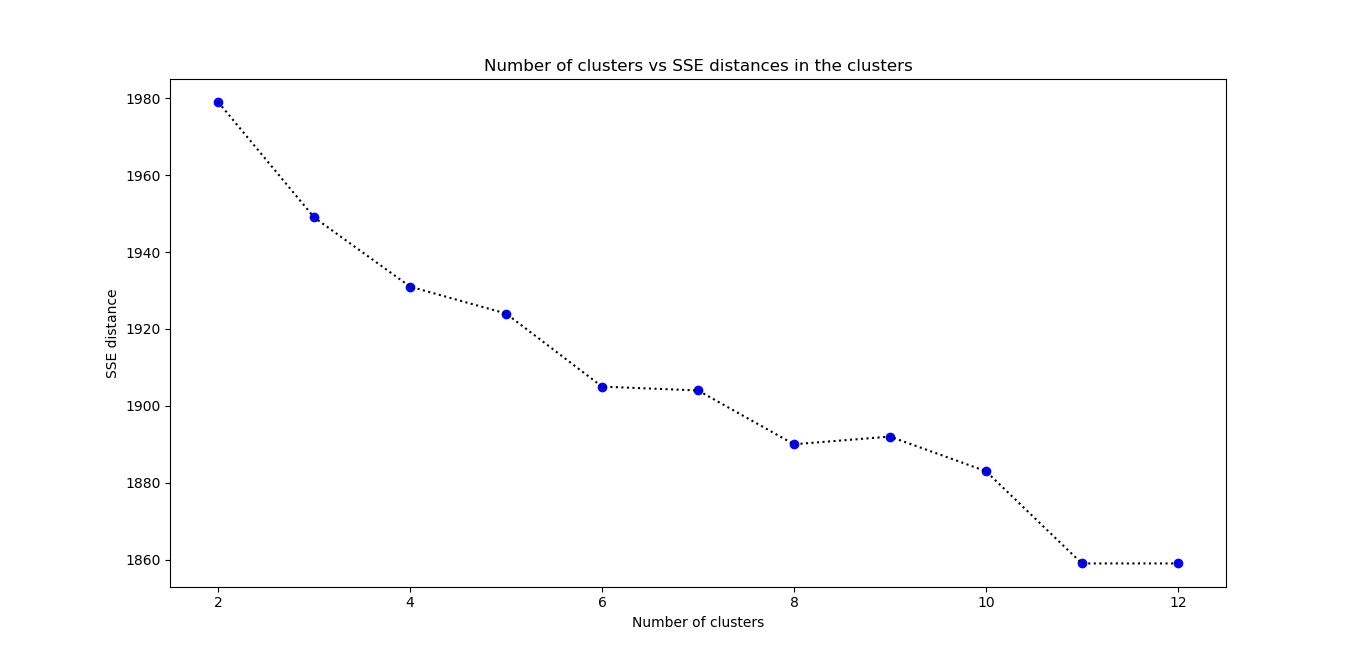
\includegraphics[width=1\linewidth]{./img/kmeans_elbow.png}
    \end{subfigure}    
    \caption{Elbow method for number of cluster vs cost function (SSE distance)}
    \label{fig:elbow}
\end{figure}

As is clearly visible, by applying the Elbow method, we have decided to work with a number of cluster of \textbf{K=8}.

The code that shows what is explained above is presented in here: 

CODE OF NOISE REMOVAL

Before jumping to the application of k-means for 8 clusters, we have applied the consensus Matrix as a method of noise removal, to determine the tweets that do not fit properly in a cluster for different
values of K (from 2 to 12). To do so, we have applied the code in the listing \ref{lst:Consensus implementation}. Additionally in the line 19, the pair of tweets that are pair less than a 10\% (less than one time) is not taken into account.
\begin{lstlisting}[language=Python, caption= Consensus Algorithm, label={lst:Consensus implementation}]
    import numpy as np
    from csv_helper import CSVHelper
    
    c_matrix = np.zeros((2001,2001), dtype=int)
    print(c_matrix.shape)
    
    for i in range(11):
        list_clasification = CSVHelper.load_csv("k"+str(i+2)+".csv")
        for x, val1 in enumerate(list_clasification):
            for y, val2 in enumerate(list_clasification):
                if val1 == val2:
                    c_matrix[x][y] += 1
    
    print(c_matrix)
    np.savetxt("conse.csv", c_matrix, fmt='%i',delimiter=",")

    # Removing extra noise for tweets paired less than a 10%
    consensus = np.loadtxt(open("conse.csv", "rb"), delimiter=",", skiprows=0)
    consensus[consensus == 1] = 0
\end{lstlisting}

Once the Consensus Matrix is build, the next step is calculate the Noise tweet by comparing the tweets implication with the average total implications in the entire matrix by using the following code:

\begin{lstlisting}[language=Python, caption= Consensus Noise, label={lst:Consensus_Noise}]
consensus = np.loadtxt(open("conse.csv", "rb"), delimiter=",", skiprows=0)
consensus[consensus == 1] = 0

def get_average(matrix):
    sum = 0
    count = 0
    for i in range(matrix.shape[0]):
        for j in range(matrix.shape[0]):
            if i != j:
                sum += matrix[i][j]
                count += 1
    return (sum/count)
            

print(consensus[0,:])

def get_noise_list(matrix):
    noise_list=[]
    for i in range(matrix.shape[0]):
        row = consensus[i,:]
        summatory = sum(row)
        avg = (summatory - 11)/2000
        if avg < 6.882:
            noise_list.append(i)
    return noise_list

res = get_noise_list(consensus)
\end{lstlisting}

This results in the classification of \textit{848} tweets as noise. This tweets will be later removed from the clustered tweets for the \textbf{K=8} obtained previously
by the elbow method.

With the removal of the noise tweets in the previous cluster, it basically disapered six cluster, leaving the \textbf{K=8} into a \textbf{K=2}.

\subsection{DBSCAN}
            
The other algorithm we needed to implement was DBSCAN. As we have already seen during the lectures, DBSCAN requires two parameters: the
radius $\epsilon$ and the minimum number of points required to form a dense region (minPts). Initially no point has been visited so we start 
randomly by one point. What we do next in the algorithm is to retrieve the number of neighbor nodes within $\epsilon$ distance to later decide if the point 
contains sufficiently points to be considered as a core node or if it noise.

There is also a expand cluster method that will add nodes and another cluster that could be directly or indirectly reached by the cluster. For the implementation of DBSCAN we decided to do it by writing our 
own code implementation, having as a reference the code that was provided during the lab session. Similarly to what we did for K-Means, we ran the algorithms many times by changing $\epsilon$ and the \textit{minPts} in four different scenarios presented in the figure \ref{fig:dbresults}. It 
includes \textit{(a)} where $\epsilon$ is fixed to 0.5 and the  \textit{minPts} is incremented, a case \textit{(b)} incrementing $\epsilon$ and fixing \textit{minPts} to 5, the third case \textit{(c)} where $\epsilon$ is also incremented and \textit{minPts} is fixed to 5. Finally, a scenario \textit{(d)} where 
both parameters are incremented.

The intention behind this "scenarios" changing the parameters, is to somehow follow a Sensitivity Analysis for the expected output "number of clusters". Due to the fact that we could not find a direct or linear relation between the inputs ($\epsilon$ and \textit{minPts}) and the \textit{number of clusters}, we did a qualitative
result among all the scenarios to choose the pair of inputs that provide a "fair" (balanced or middle point in between the option) with not more than a 40\% of nodes considered as noise.

Following this logic, we found that a middle value that respected our previous conditions is when $\epsilon$ is 0.8 and \textit{minPts} is 10. This give us a total of \textbf{7} \textit{clusters} and \textbf{781} tweets considered as noise (less than 40\%).

\begin{figure}[H]
    \centering 
    \begin{subfigure}{1\textwidth}  
        \begin{subfigure}{.5\textwidth}
            \centering   
            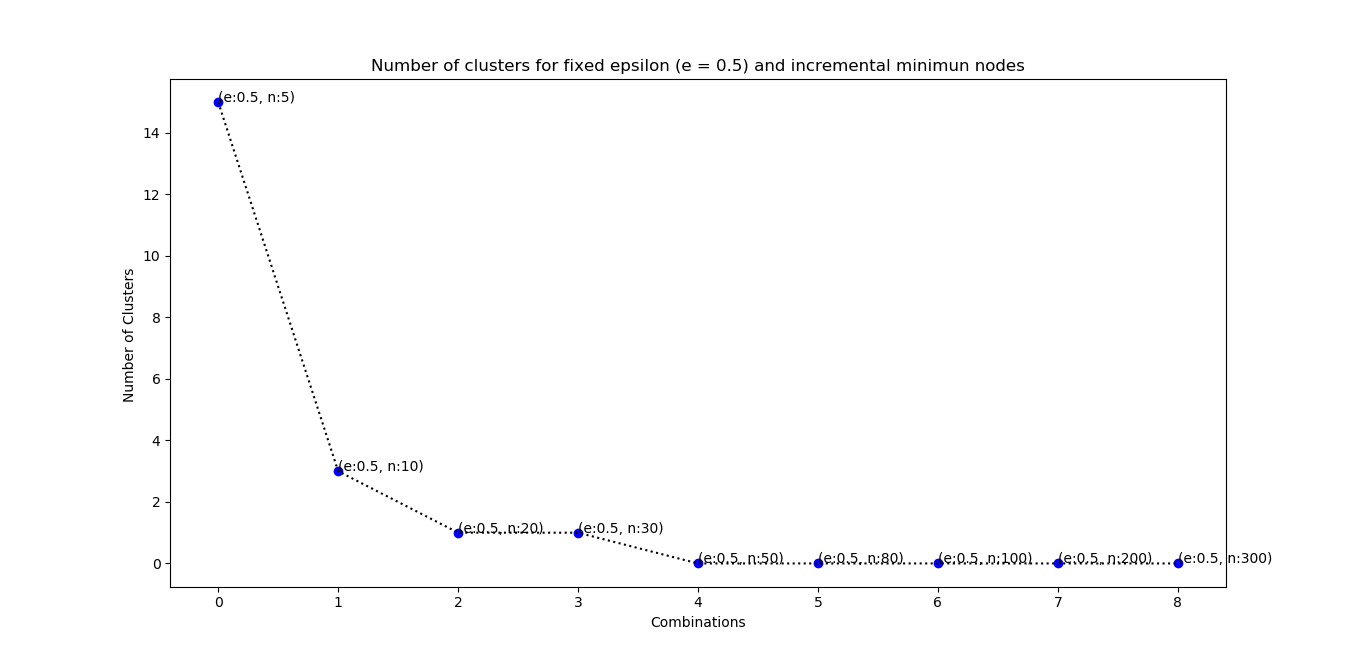
\includegraphics[width=1\linewidth]{./img/e0-5n.png}
            \caption{ }
        \end{subfigure}
        \begin{subfigure}{.5\textwidth}  
            \centering 
            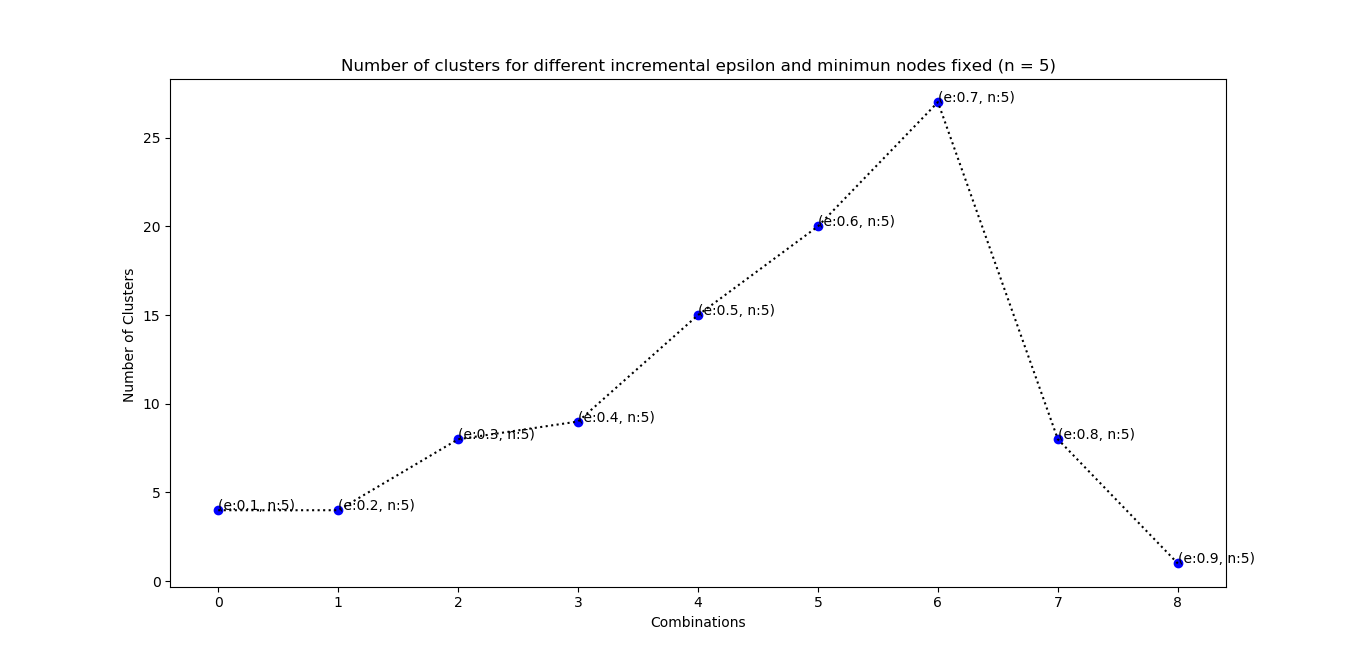
\includegraphics[width=1\linewidth]{./img/en5.png}
            \caption{}
        \end{subfigure}
        \begin{subfigure}{.5\textwidth} 
            \centering  
            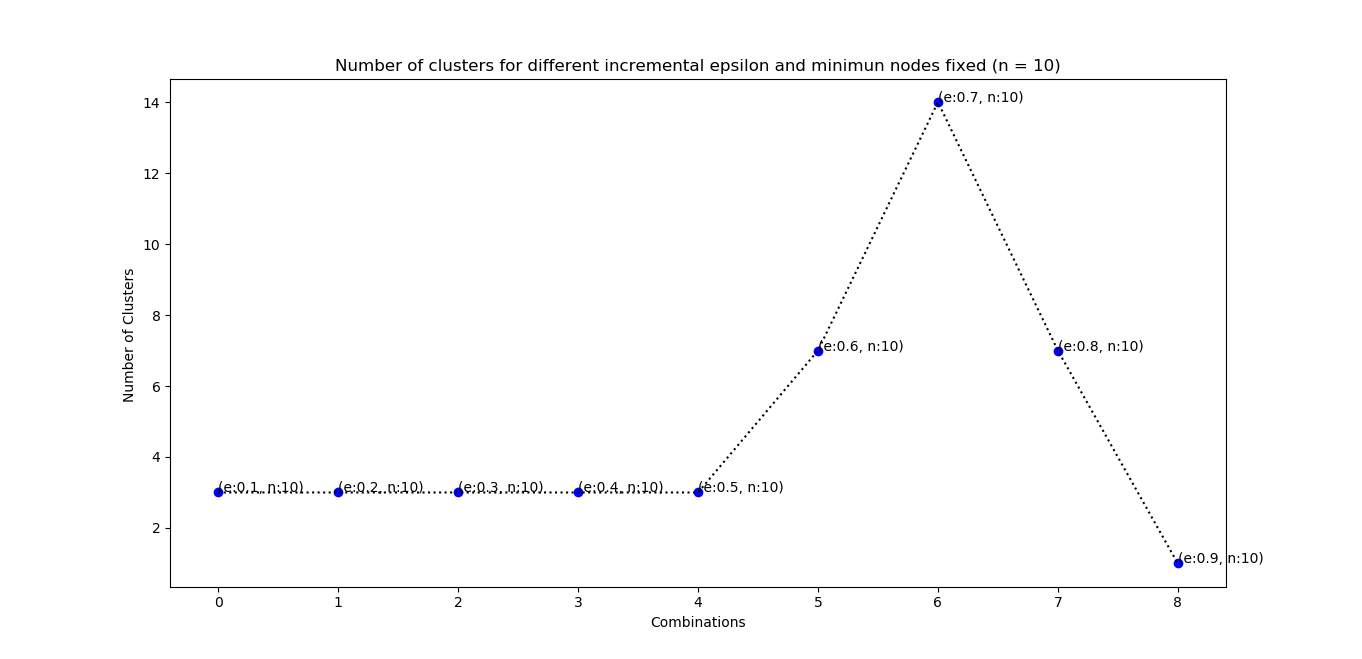
\includegraphics[width=1\linewidth]{./img/en10.png}
            \caption{}
        \end{subfigure}
        \begin{subfigure}{.5\textwidth} 
            \centering  
            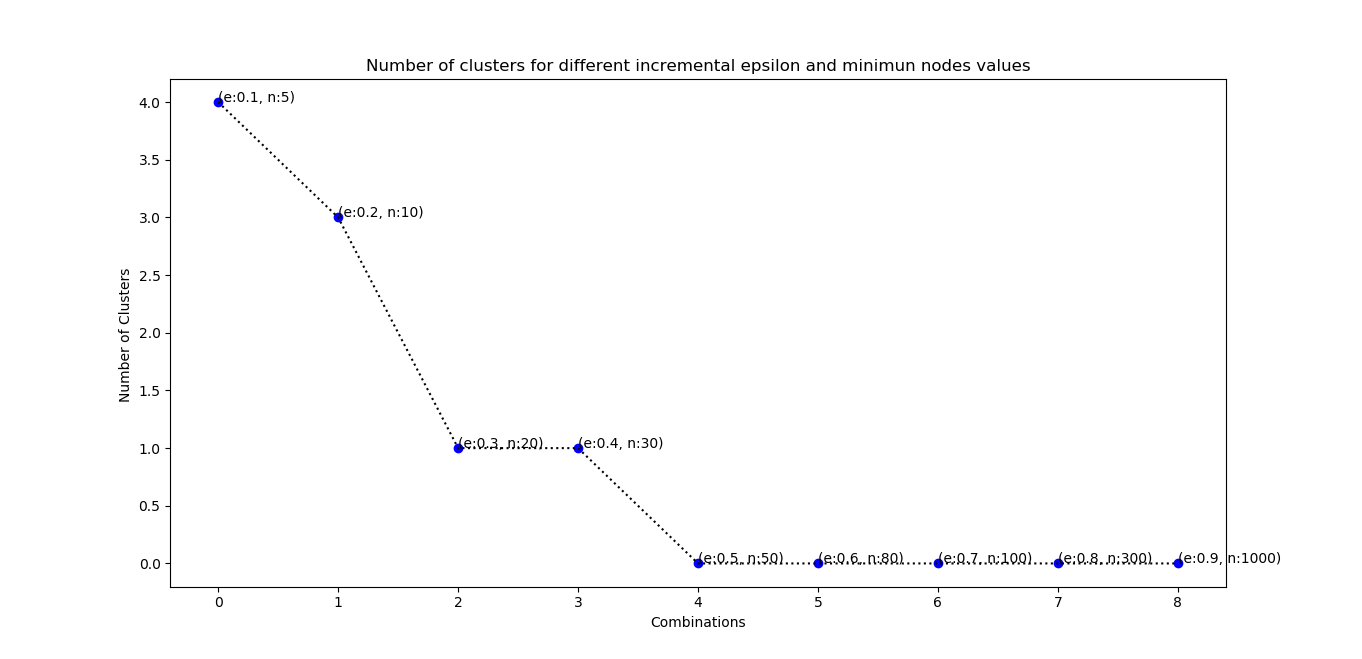
\includegraphics[width=1\linewidth]{./img/inc.png}
            \caption{}
        \end{subfigure}                
    \end{subfigure}
    \caption{DBSCAN Number of cluster results for different Epsilon and minnodes values}
    \label{fig:dbresults}
\end{figure}

CODE FOR DBSCANN
\begin{lstlisting}[language=Python, caption= DBSCAN Algorithm, label={lst:DBSCAN implementation}]
def DBSCAN(matrix, epsilon, min_nodes):
    print('epsilon', epsilon)
    print('mnodes', min_nodes)
    noise = []
    visited = []
    clusters = []
    c_n = -1 #cluster number or position
    for node in matrix:
        if node[1] not in visited:
            visited.append(node[1])
            neighbour_nodes = regionScan(node[1], epsilon, matrix)
            if len(neighbour_nodes) < min_nodes:
                print('adding noise')
                noise.append(node[1])
            else:
                clusters.append([])
                c_n += 1
                expandCluster(node, neighbour_nodes, clusters, c_n,epsilon, min_nodes, matrix, visited)
    print("no. of clusters: " , len(clusters))
    print("length of noise:", len(noise))
    print("clusters " , clusters)
    print("noise " , noise)
            
            \end{lstlisting}

\newpage
\section{Clustering}
        
Since now we have the final clustering for each dataset (DBSCAN and K-means), we count for each cluster which is the most frequent word. To do so, we need to go through the words present in each tweets for a corresponding cluster and count how many times they are repeating and finding the one that is repetead more. The code below describes the procedure we followed. 

\begin{lstlisting}[language=Python, caption= Mostly used word/cluster, label={lst:Mostly used word/cluster}]
resultWords = []
for x,cluster in enumerate(listDoc):
    scores = {}
    blobList = reduce(lambda x,y: x+y,cluster)
    for i, blob in enumerate(cluster):
        scores = {word: tf(word, blobList) for word in blob.words}
        sorted_words = sorted(scores.items(), key=lambda x: x[1], reverse=True)
    resultWords.append({'cluster'+str(x): sorted_words[0][0]})
    print(sorted_words)
print(resultWords)
 \end{lstlisting}

The results of the most frequent word in each cluster for each method is presented in the \ref{fig:table}.

\begin{figure}[H]
    \centering 
    \begin{subfigure}{1\textwidth}  
        \begin{subfigure}{.5\textwidth}
            \centering   
            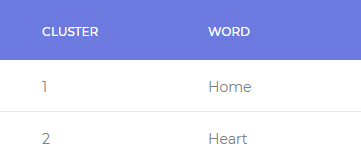
\includegraphics[width=.8\linewidth]{./img/kmeantb.jpg}
            \caption{K-MEANS}
        \end{subfigure}
        \begin{subfigure}{.5\textwidth}  
            \centering 
            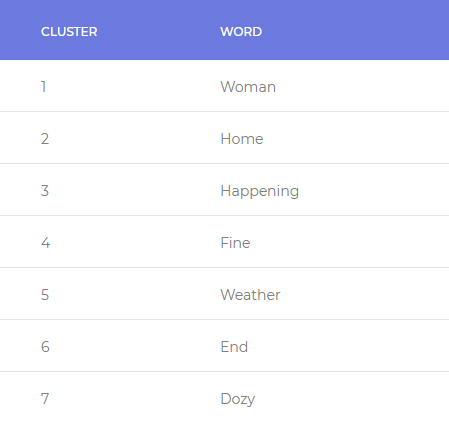
\includegraphics[width=1\linewidth]{./img/dbscantb.jpg}
            \caption{DBSCAN}
        \end{subfigure}                
    \end{subfigure}
    \caption{Most frequent word by cluster for K-means and DBSCAN results}
    \label{fig:table}
\end{figure}

\newpage
\section{Visualization}
        
For both implementations,we have visualized the results. We have used the graphing software Gephi as suggested.
To create the graphs based on the results of the clustering, we imported the 2 csv files to each project, one with the node lists and one with the edges in between. 
We repeated this step twice for the 2 different results that we got after running 
K-means and DBSCAN.


K-means Result image visualization

\begin{figure}[H]
    \begin{subfigure} {1\textwidth}  
        \centering 
        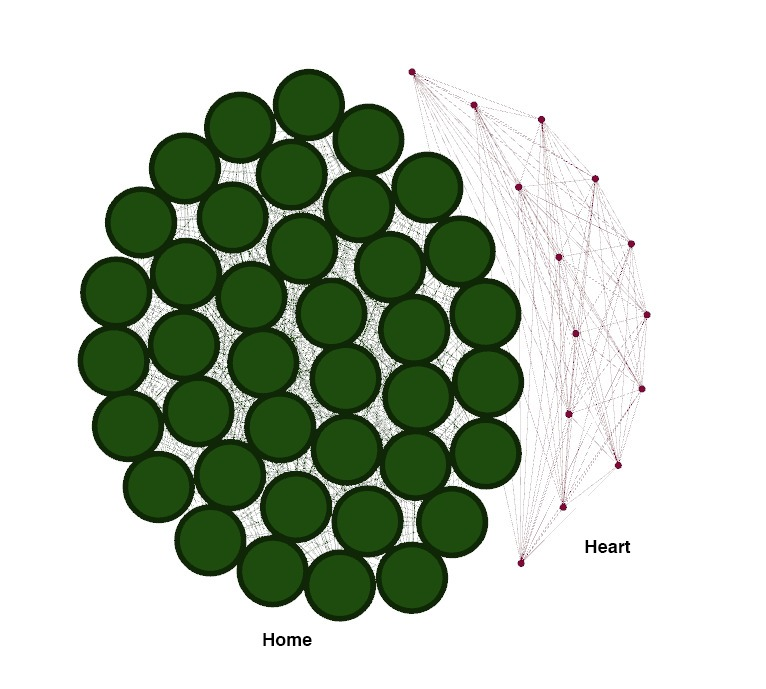
\includegraphics[width=0.6\linewidth]{./img/kmeans.jpeg}
    \end{subfigure}    
    \caption{Results for K-means clustering after removing noise}
    \label{fig:movement}
\end{figure}

DBSCAN Result image Visualization

\begin{figure}[H]
    \begin{subfigure} {1\textwidth}  
        \centering 
        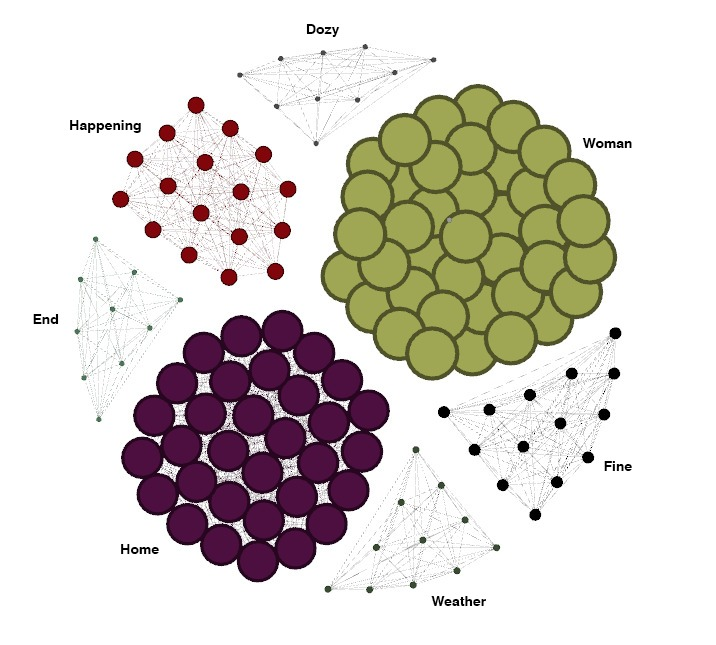
\includegraphics[width=0.6\linewidth]{./img/dbscan.jpeg}
    \end{subfigure}    
    \caption{Results for DBSCAN epsilon: 0.8 and minnodes: 10}
    \label{fig:movement}
\end{figure}


\newpage
\section{Conclusion}
The knowledge that we got at the end of this project, made us to have a real-life approach of how to do data representation, reduction and analysis. Even if we learned a lot of data cleaning techniques for our Distributing Computing and Storage Architecture project, in this project we expanded our knowledge more by learning more pre-processing techniques. 

After having successfully understood the K-Means and DBSCAN algorithm, doing the implementation for the dataset that we had was not that easy. We faced many issues and difficulties that you experience only if you have a real-life scenario and this is also the reason why we have appreciated and learned so much from this.


\newpage
\bibliography{report}
\bibliographystyle{ieeetr}
\nocite{*}
\end{document}